\documentclass[11pt,a4paper]{article}

%% ─── Packages ────────────────────────────────────────────────────────────────
\usepackage[margin=2.5cm]{geometry}
\usepackage[T1]{fontenc}
\usepackage[utf8]{inputenc}
\usepackage{lmodern}
\usepackage{xcolor}
\usepackage{tikz}
\usetikzlibrary{arrows.meta,positioning,shapes.geometric,fit,calc,backgrounds,decorations.pathreplacing}
\usepackage{listings}
\usepackage{booktabs}
\usepackage{tabularx}
\usepackage{longtable}
\usepackage{array}
\usepackage{fancyhdr}
\usepackage{titlesec}
\usepackage{hyperref}
\usepackage{enumitem}
\usepackage{mdframed}
\usepackage{multirow}

%% ─── Fix headheight warning ──────────────────────────────────────────────────
\setlength{\headheight}{14pt}

%% ─── Color Palette ───────────────────────────────────────────────────────────
\definecolor{green}{HTML}{2EA043}
\definecolor{cyan}{HTML}{58A6FF}
\definecolor{amber}{HTML}{D29922}
\definecolor{red}{HTML}{DA3633}
\definecolor{border}{HTML}{30363D}
\definecolor{textmuted}{HTML}{6E7681}
\definecolor{sectionblue}{HTML}{1F6FEB}
\definecolor{accentpurple}{HTML}{8957E5}
\definecolor{lightgray}{HTML}{F6F8FA}
\definecolor{darkgray}{HTML}{21262D}

%% ─── Hyperref ────────────────────────────────────────────────────────────────
\hypersetup{
  colorlinks=true,
  linkcolor=sectionblue,
  urlcolor=sectionblue,
  pdftitle={ARES CTI Dashboard -- Technical Documentation},
  pdfauthor={Rafael Rodriguez},
}

%% ─── Section Styling ─────────────────────────────────────────────────────────
\titleformat{\section}{\Large\bfseries\color{sectionblue}}{}{0em}{}[\color{border}\titlerule]
\titleformat{\subsection}{\large\bfseries\color{darkgray}}{}{0em}{}
\titleformat{\subsubsection}{\normalsize\bfseries\color{textmuted}}{}{0em}{}

%% ─── Header / Footer ─────────────────────────────────────────────────────────
\pagestyle{fancy}
\fancyhf{}
\fancyhead[L]{\small\color{textmuted}ARES CTI Dashboard}
\fancyhead[R]{\small\color{textmuted}Technical Documentation}
\fancyfoot[C]{\small\color{textmuted}\thepage}
\renewcommand{\headrulewidth}{0.4pt}

%% ─── Code Listings ───────────────────────────────────────────────────────────
\lstdefinelanguage{json}{
  basicstyle=\ttfamily\small,
  morestring=[b]",
  stringstyle=\color{green!60!black},
  literate=
   *{0}{{{\color{sectionblue}0}}}{1}
    {1}{{{\color{sectionblue}1}}}{1}
    {2}{{{\color{sectionblue}2}}}{1}
    {3}{{{\color{sectionblue}3}}}{1}
    {4}{{{\color{sectionblue}4}}}{1}
    {5}{{{\color{sectionblue}5}}}{1}
    {6}{{{\color{sectionblue}6}}}{1}
    {7}{{{\color{sectionblue}7}}}{1}
    {8}{{{\color{sectionblue}8}}}{1}
    {9}{{{\color{sectionblue}9}}}{1},
}
\lstdefinestyle{code}{
  backgroundcolor=\color{lightgray},
  basicstyle=\ttfamily\small,
  keywordstyle=\color{sectionblue}\bfseries,
  stringstyle=\color{green!60!black},
  commentstyle=\color{textmuted}\itshape,
  breaklines=true,
  frame=single,
  framesep=4pt,
  rulecolor=\color{border},
  xleftmargin=8pt,
  xrightmargin=8pt,
  showstringspaces=false,
  numbers=none,
}
\lstset{style=code}

%% ─── Custom Boxes ────────────────────────────────────────────────────────────
\newmdenv[
  linecolor=green,linewidth=1.5pt,
  leftline=true,rightline=false,topline=false,bottomline=false,
  leftmargin=0pt,rightmargin=0pt,
  innerleftmargin=10pt,innerrightmargin=6pt,
  innertopmargin=6pt,innerbottommargin=6pt,
  backgroundcolor=green!5,
]{greenbox}

\newmdenv[
  linecolor=amber,linewidth=1.5pt,
  leftline=true,rightline=false,topline=false,bottomline=false,
  leftmargin=0pt,rightmargin=0pt,
  innerleftmargin=10pt,innerrightmargin=6pt,
  innertopmargin=6pt,innerbottommargin=6pt,
  backgroundcolor=amber!5,
]{amberbox}

\newmdenv[
  linecolor=red,linewidth=1.5pt,
  leftline=true,rightline=false,topline=false,bottomline=false,
  leftmargin=0pt,rightmargin=0pt,
  innerleftmargin=10pt,innerrightmargin=6pt,
  innertopmargin=6pt,innerbottommargin=6pt,
  backgroundcolor=red!5,
]{redbox}

\newmdenv[
  linecolor=sectionblue,linewidth=1.5pt,
  leftline=true,rightline=false,topline=false,bottomline=false,
  leftmargin=0pt,rightmargin=0pt,
  innerleftmargin=10pt,innerrightmargin=6pt,
  innertopmargin=6pt,innerbottommargin=6pt,
  backgroundcolor=sectionblue!5,
]{bluebox}

%% ─── TikZ Styles ─────────────────────────────────────────────────────────────
\tikzset{
  mynode/.style={
    draw=#1!70!black, fill=#1!10, rounded corners=4pt,
    font=\small\bfseries, align=center,
    inner sep=6pt,
  },
  arrow/.style={-{Stealth[length=6pt]}, thick, color=border},
  drarrow/.style={-{Stealth[length=6pt]}, thick, color=border, dashed},
  lbl/.style={font=\scriptsize\itshape, color=textmuted, midway},
}

%% ─────────────────────────────────────────────────────────────────────────────
\begin{document}

%% ─── Title Page ──────────────────────────────────────────────────────────────
\begin{titlepage}
\centering
\vspace*{2.5cm}

{\Huge\bfseries\color{sectionblue} ARES CTI Dashboard}\\[12pt]
{\Large\color{textmuted} Cyber Threat Intelligence Aggregation Platform}\\[0.5cm]
\textcolor{border}{\rule{10cm}{0.4pt}}\\[0.5cm]
{\large Technical Documentation \& Architecture Reference}\\[1.5cm]

\begin{tabular}{ll}
\textbf{Author}  & Rafael Rodriguez \\[4pt]
\textbf{Stack}   & Python / Flask \quad React / TypeScript / Vite \\[4pt]
\textbf{Date}    & April 2026 \\[4pt]
\textbf{Version} & 1.0.0 \\
\end{tabular}

\vspace{2cm}
\begin{mdframed}[linecolor=border,linewidth=1pt,roundcorner=6pt,
                 innerleftmargin=20pt,innerrightmargin=20pt,
                 innertopmargin=12pt,innerbottommargin=12pt]
\centering
Aggregates threat intelligence from \textbf{AbuseIPDB}, \textbf{AlienVault OTX}, and \textbf{VirusTotal}\\
into a unified analyst-facing dashboard with IOC lookup, scoring, and live feeds.
\end{mdframed}

\end{titlepage}

\tableofcontents
\newpage

%% ═══════════════════════════════════════════════════════════════════════════
\section{Executive Summary}

ARES CTI Dashboard is a full-stack web application that aggregates \textbf{Cyber Threat Intelligence (CTI)} from three industry-standard APIs:
\textbf{AbuseIPDB}, \textbf{AlienVault OTX}, and \textbf{VirusTotal}. It gives security analysts a single pane of glass to:

\begin{itemize}[leftmargin=1.5cm]
  \item Look up any \textbf{Indicator of Compromise (IOC)} — IP address, domain, or file hash — and receive an aggregated risk score (0--100) from multiple sources.
  \item Browse a live \textbf{threat intelligence feed} from AlienVault OTX subscribed pulses.
  \item Monitor the \textbf{health} of all integrated data sources in real time.
  \item Review raw API responses per source for deeper analyst investigation.
\end{itemize}

\begin{bluebox}
\textbf{Project motivation:} Most CTI tools require switching between multiple browser tabs and platforms. ARES collapses that into one dashboard, normalises risk scores to a common 0--100 scale, and caches results so analysts are not burning through API rate limits on repeated lookups.
\end{bluebox}

\subsection*{Key Numbers at a Glance}

\begin{center}
\begin{tabular}{lll}
\toprule
\textbf{Dimension} & \textbf{Value} & \textbf{Notes} \\
\midrule
External APIs integrated & 3 & AbuseIPDB, AlienVault OTX, VirusTotal \\
IOC types supported & 3 & IP, Domain, File Hash \\
Bulk lookup limit & 50 IOCs & Parallelised via ThreadPoolExecutor \\
Cache TTL (indicators) & 60 min & Prevents redundant upstream calls \\
Cache TTL (feed) & 5 min & Near-real-time pulse freshness \\
API endpoints & 8 & Health, indicators, bulk, feed, stats \\
Frontend pages & 3 & Dashboard, Lookup, Feed \\
\bottomrule
\end{tabular}
\end{center}

\newpage

%% ═══════════════════════════════════════════════════════════════════════════
\section{What the App Does}

\subsection{Core Features}

\subsubsection{IOC Lookup}
An analyst types an IP address (\texttt{1.2.3.4}), domain (\texttt{evil.com}), or file hash (\texttt{d41d8cd9...}) into the search bar. The app auto-detects the IOC type using regex, then fans out \textbf{parallel requests} to all relevant threat intelligence sources. The analyst sees:

\begin{itemize}
  \item A \textbf{circular risk gauge} coloured green / amber / red
  \item Aggregated metadata: country of origin, last-seen timestamp, contributing sources
  \item Deduplicated \textbf{threat tags} across all sources
  \item A \textbf{per-source breakdown} panel
  \item Toggle to expose the \textbf{raw JSON} from each source
\end{itemize}

\subsubsection{Threat Feed}
The Feed page pulls from AlienVault OTX subscribed pulses -- community-curated threat reports. The analyst sees a table of pulses with name, author, tags, indicator count, and creation date. The feed auto-refreshes every 5 minutes.

\subsubsection{Dashboard Overview}
The landing page surfaces aggregated stats, a horizontal bar chart of the top 10 threat tags (Recharts), source health status, and a recent pulses summary table.

\subsubsection{Bulk Lookup (API-first)}
A POST endpoint (\texttt{/api/indicators/bulk}) accepts up to 50 IOCs and processes them in parallel threads, returning a map of IOC to result. No UI yet -- ready for scripting and automation workflows.

\newpage

%% ═══════════════════════════════════════════════════════════════════════════
\section{System Architecture}

\subsection{High-Level Architecture}

\begin{center}
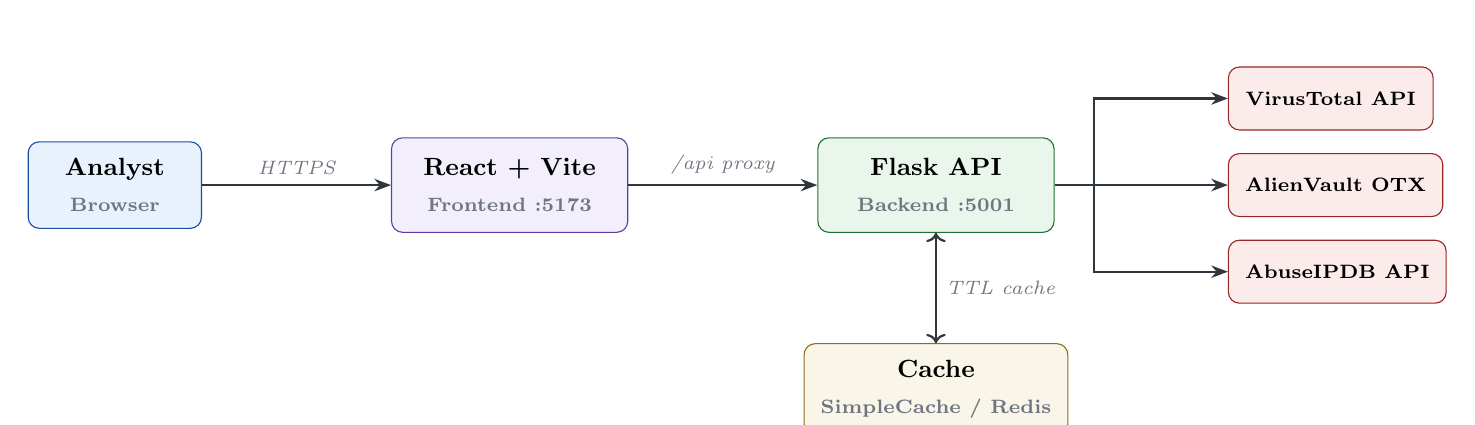
\begin{tikzpicture}[node distance=1.6cm and 2.4cm]

  \node[mynode=sectionblue,
        minimum width=2.2cm, minimum height=1cm] (analyst)
    {\small\bfseries Analyst\\[2pt]{\scriptsize\color{textmuted}Browser}};

  \node[mynode=accentpurple,
        minimum width=3cm, minimum height=1.2cm,
        right=2.4cm of analyst] (fe)
    {\small\bfseries React + Vite\\[2pt]{\scriptsize\color{textmuted}Frontend :5173}};

  \node[mynode=green,
        minimum width=3cm, minimum height=1.2cm,
        right=2.4cm of fe] (be)
    {\small\bfseries Flask API\\[2pt]{\scriptsize\color{textmuted}Backend :5001}};

  \node[mynode=amber,
        minimum width=2.4cm, minimum height=0.9cm,
        below=1.4cm of be] (cache)
    {\small Cache\\[2pt]{\scriptsize\color{textmuted}SimpleCache / Redis}};

  \node[mynode=red,
        minimum width=2.6cm, minimum height=0.8cm,
        right=2.2cm of be, yshift=1.1cm] (vt)
    {\scriptsize VirusTotal API};

  \node[mynode=red,
        minimum width=2.6cm, minimum height=0.8cm,
        right=2.2cm of be] (av)
    {\scriptsize AlienVault OTX};

  \node[mynode=red,
        minimum width=2.6cm, minimum height=0.8cm,
        right=2.2cm of be, yshift=-1.1cm] (ab)
    {\scriptsize AbuseIPDB API};

  \draw[arrow] (analyst) -- node[lbl,above]{HTTPS} (fe);
  \draw[arrow] (fe)      -- node[lbl,above]{/api proxy} (be);
  \draw[arrow,<->] (be)  -- node[lbl,right]{TTL cache} (cache);
  \draw[arrow] (be.east) -- ++(0.5,0) |- (vt.west);
  \draw[arrow] (be.east) -- ++(0.5,0) -- (av.west);
  \draw[arrow] (be.east) -- ++(0.5,0) |- (ab.west);

\end{tikzpicture}
\end{center}

\vspace{0.4cm}

\subsection{Backend Architecture -- Flask Blueprints}

\begin{center}
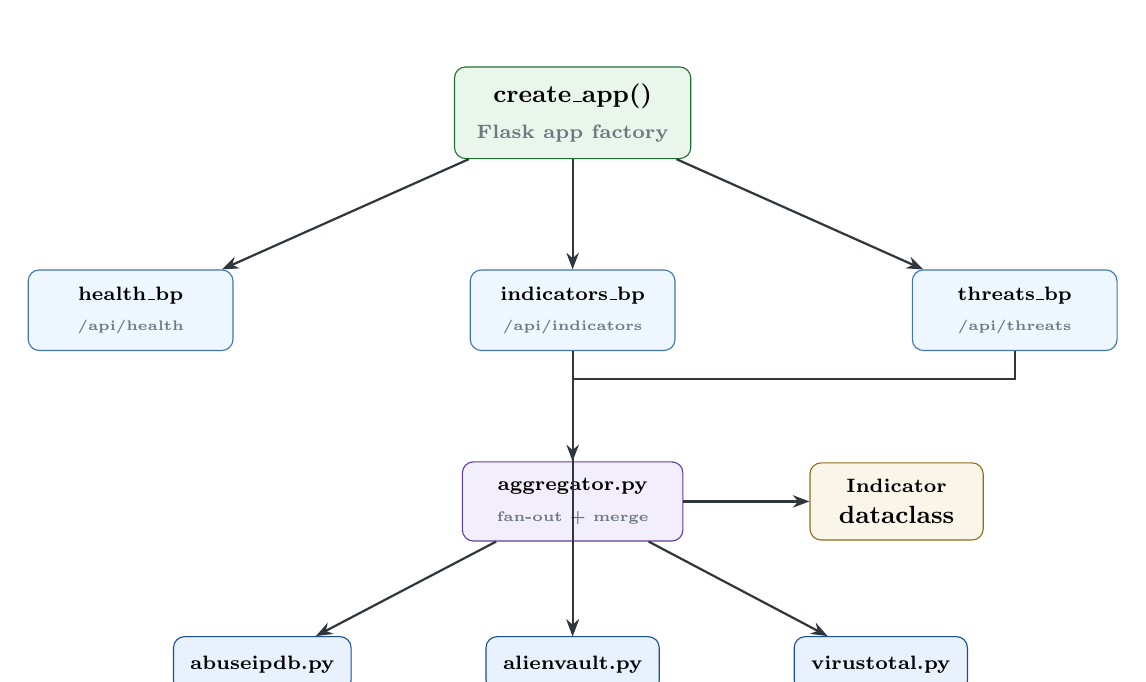
\begin{tikzpicture}[node distance=1.1cm and 1.8cm]

  \node[mynode=green, minimum width=3cm, minimum height=0.9cm] (factory)
    {\small create\_app()\\[2pt]{\scriptsize\color{textmuted}Flask app factory}};

  \node[mynode=cyan, minimum width=2.6cm, minimum height=0.8cm,
        below left=1.4cm and 2.8cm of factory] (bp1)
    {\scriptsize health\_bp\\{\tiny\color{textmuted}/api/health}};

  \node[mynode=cyan, minimum width=2.6cm, minimum height=0.8cm,
        below=1.4cm of factory] (bp2)
    {\scriptsize indicators\_bp\\{\tiny\color{textmuted}/api/indicators}};

  \node[mynode=cyan, minimum width=2.6cm, minimum height=0.8cm,
        below right=1.4cm and 2.8cm of factory] (bp3)
    {\scriptsize threats\_bp\\{\tiny\color{textmuted}/api/threats}};

  \node[mynode=accentpurple, minimum width=2.8cm, minimum height=0.8cm,
        below=1.4cm of bp2] (agg)
    {\scriptsize aggregator.py\\{\tiny\color{textmuted}fan-out + merge}};

  \node[mynode=sectionblue, minimum width=2.2cm, minimum height=0.7cm,
        below left=1.2cm and 1.4cm of agg] (s1)
    {\scriptsize abuseipdb.py};

  \node[mynode=sectionblue, minimum width=2.2cm, minimum height=0.7cm,
        below=1.2cm of agg] (s2)
    {\scriptsize alienvault.py};

  \node[mynode=sectionblue, minimum width=2.2cm, minimum height=0.7cm,
        below right=1.2cm and 1.4cm of agg] (s3)
    {\scriptsize virustotal.py};

  \node[mynode=amber, minimum width=2.2cm, minimum height=0.7cm,
        right=1.6cm of agg] (model)
    {\scriptsize Indicator\\dataclass};

  \draw[arrow] (factory) -- (bp1);
  \draw[arrow] (factory) -- (bp2);
  \draw[arrow] (factory) -- (bp3);
  \draw[arrow] (bp2) -- (agg);
  \draw[arrow] (bp3.south) -- ++(0,-0.35) -| (s2.north);
  \draw[arrow] (agg) -- (s1);
  \draw[arrow] (agg) -- (s2);
  \draw[arrow] (agg) -- (s3);
  \draw[arrow] (agg) -- (model);

\end{tikzpicture}
\end{center}

\newpage

\subsection{Frontend Architecture -- React Component Tree}

\begin{center}
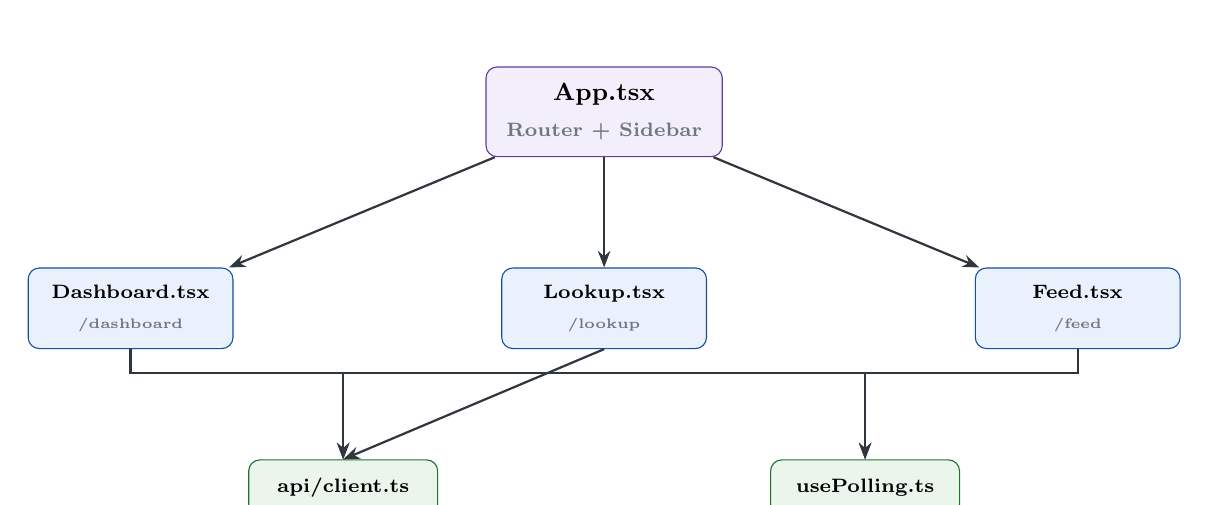
\begin{tikzpicture}[node distance=1.1cm and 2cm]

  \node[mynode=accentpurple, minimum width=3cm, minimum height=0.9cm] (app)
    {\small App.tsx\\[2pt]{\scriptsize\color{textmuted}Router + Sidebar}};

  \node[mynode=sectionblue, minimum width=2.6cm, minimum height=0.8cm,
        below left=1.4cm and 3.2cm of app] (dash)
    {\scriptsize Dashboard.tsx\\{\tiny\color{textmuted}/dashboard}};

  \node[mynode=sectionblue, minimum width=2.6cm, minimum height=0.8cm,
        below=1.4cm of app] (look)
    {\scriptsize Lookup.tsx\\{\tiny\color{textmuted}/lookup}};

  \node[mynode=sectionblue, minimum width=2.6cm, minimum height=0.8cm,
        below right=1.4cm and 3.2cm of app] (feed)
    {\scriptsize Feed.tsx\\{\tiny\color{textmuted}/feed}};

  \node[mynode=green, minimum width=2.4cm, minimum height=0.7cm,
        below left=1.4cm and 0.8cm of look] (client)
    {\scriptsize api/client.ts};

  \node[mynode=green, minimum width=2.4cm, minimum height=0.7cm,
        below right=1.4cm and 0.8cm of look] (hook)
    {\scriptsize usePolling.ts};

  \draw[arrow] (app) -- (dash);
  \draw[arrow] (app) -- (look);
  \draw[arrow] (app) -- (feed);
  \draw[arrow] (dash.south) -- ++(0,-0.3) -| (client.north);
  \draw[arrow] (look.south) -- (client.north);
  \draw[arrow] (feed.south) -- ++(0,-0.3) -| (client.north);
  \draw[arrow] (dash.south) -- ++(0,-0.3) -| (hook.north);
  \draw[arrow] (feed.south) -- ++(0,-0.3) -| (hook.north);

\end{tikzpicture}
\end{center}

\vspace{0.5cm}

\subsection{IOC Lookup Data Flow}

\begin{center}
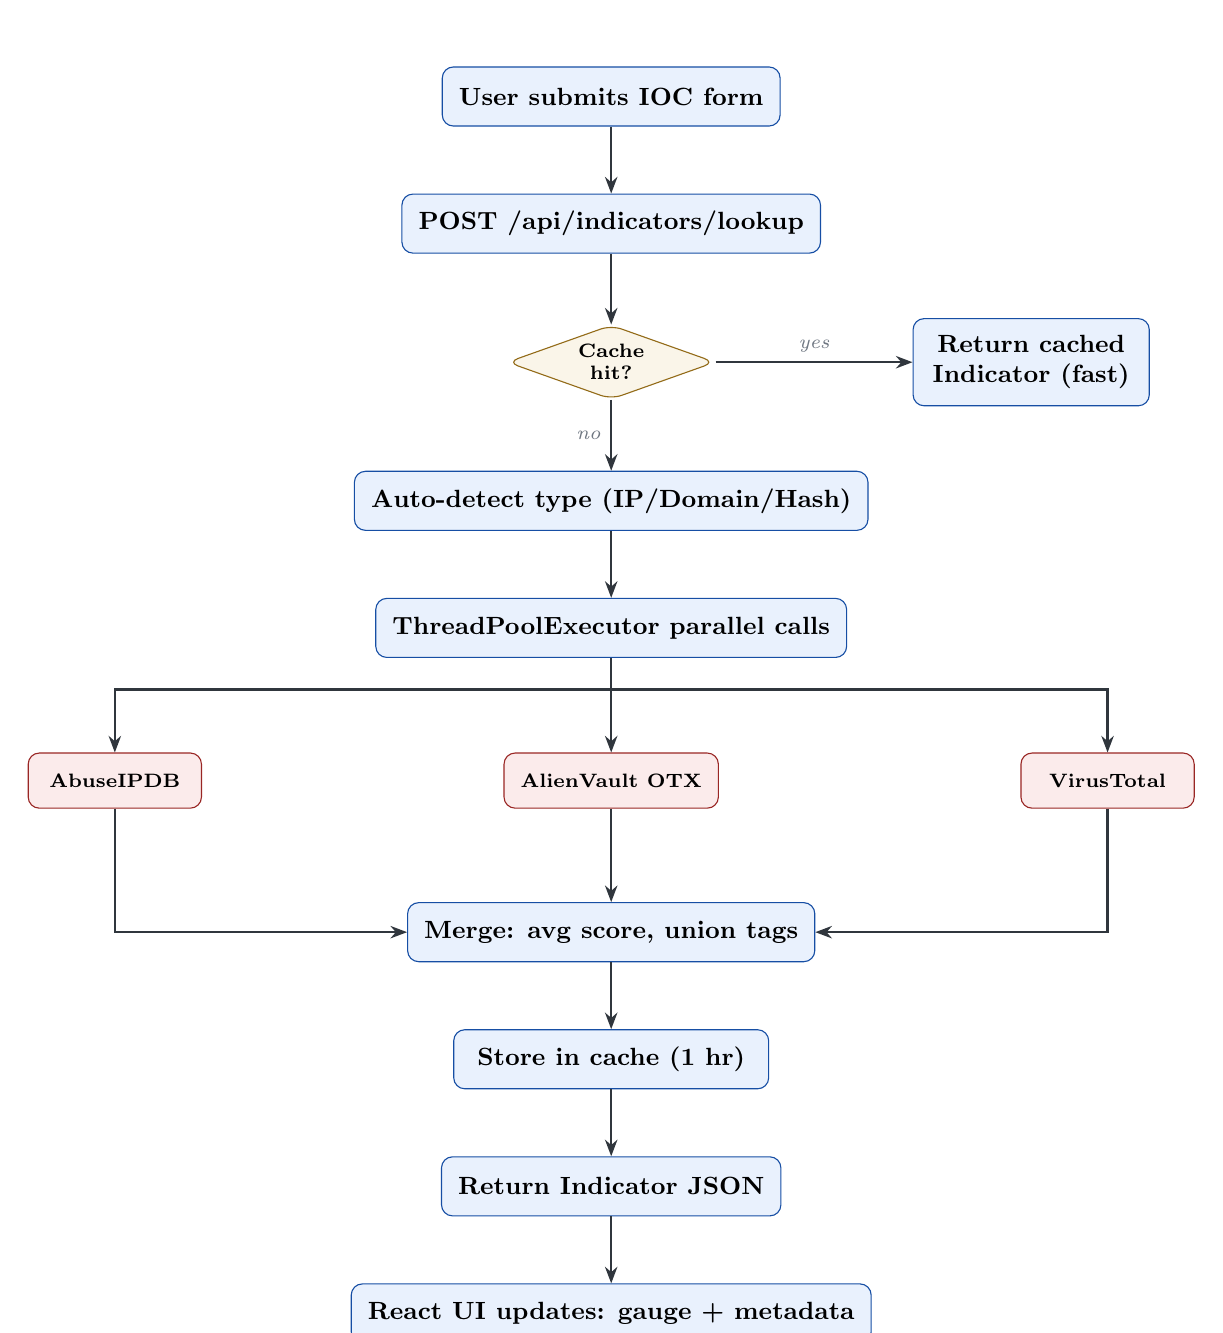
\begin{tikzpicture}[
  flowstep/.style={mynode=sectionblue, minimum width=4cm, minimum height=0.75cm},
  flowdec/.style={mynode=amber, diamond, aspect=2.8, minimum width=2cm, font=\scriptsize\bfseries, align=center, inner sep=2pt},
  flowext/.style={mynode=red, minimum width=2.2cm, minimum height=0.7cm},
  node distance=0.85cm
]

  \node[flowstep] (form) {\small User submits IOC form};
  \node[flowstep, below=of form] (post) {\small POST /api/indicators/lookup};
  \node[flowdec, below=0.9cm of post] (hit) {Cache\\hit?};
  \node[flowstep, right=2.5cm of hit, minimum width=3cm] (cached)
    {\small Return cached\\Indicator (fast)};
  \node[flowstep, below=0.9cm of hit] (detect)
    {\small Auto-detect type (IP/Domain/Hash)};
  \node[flowstep, below=of detect] (thread)
    {\small ThreadPoolExecutor parallel calls};

  \node[flowext, below left=1.2cm and 2.2cm of thread] (api1) {\scriptsize AbuseIPDB};
  \node[flowext, below=1.2cm of thread] (api2) {\scriptsize AlienVault OTX};
  \node[flowext, below right=1.2cm and 2.2cm of thread] (api3) {\scriptsize VirusTotal};

  \node[flowstep, below=3.1cm of thread] (merge)
    {\small Merge: avg score, union tags};
  \node[flowstep, below=of merge] (store) {\small Store in cache (1 hr)};
  \node[flowstep, below=of store] (resp) {\small Return Indicator JSON};
  \node[flowstep, below=of resp] (ui) {\small React UI updates: gauge + metadata};

  \draw[arrow] (form) -- (post);
  \draw[arrow] (post) -- (hit);
  \draw[arrow] (hit) -- node[lbl,left]{no} (detect);
  \draw[arrow] (hit) -- node[lbl,above]{yes} (cached);
  \draw[arrow] (detect) -- (thread);
  \draw[arrow] (thread.south) -- ++(0,-0.4) -| (api1.north);
  \draw[arrow] (thread.south) -- ++(0,-0.4) -- (api2.north);
  \draw[arrow] (thread.south) -- ++(0,-0.4) -| (api3.north);
  \draw[arrow] (api1.south) |- (merge.west);
  \draw[arrow] (api2) -- (merge);
  \draw[arrow] (api3.south) |- (merge.east);
  \draw[arrow] (merge) -- (store);
  \draw[arrow] (store) -- (resp);
  \draw[arrow] (resp) -- (ui);

\end{tikzpicture}
\end{center}

\newpage

\subsection{Caching Strategy}

\begin{center}
\begin{tabular}{llll}
\toprule
\textbf{Cache Key Pattern} & \textbf{TTL} & \textbf{Backend (dev)} & \textbf{Backend (prod)} \\
\midrule
\texttt{indicator:\{type\}:\{ioc\}} & 3600 s (1 hr) & SimpleCache & RedisCache \\
\texttt{/threats/feed?limit=N}      & 300 s (5 min) & SimpleCache & RedisCache \\
\texttt{/threats/stats}             & 600 s (10 min) & SimpleCache & RedisCache \\
\bottomrule
\end{tabular}
\end{center}

\textbf{Why these TTLs?}
\begin{itemize}
  \item \textbf{1 hour for indicators:} Threat intel for a given IOC rarely changes minute-to-minute. One hour reduces upstream API calls by $\sim$95\% for repeated lookups.
  \item \textbf{5 minutes for feed:} Threat pulses are published continuously; a short TTL keeps the feed near-real-time.
  \item \textbf{10 minutes for stats:} Aggregated tag statistics only shift meaningfully when the feed itself changes.
\end{itemize}

\newpage

%% ═══════════════════════════════════════════════════════════════════════════
\section{Design Choices \& Rationale}

\subsection{Backend: Why Flask?}

\begin{greenbox}
Flask was chosen for its \textbf{minimal footprint and explicit structure}. A CTI aggregator is fundamentally a thin proxy layer: call external APIs, merge results, cache. Flask's blueprint system maps cleanly onto this domain (one blueprint per resource group), and flask-caching plugs in without boilerplate.
\end{greenbox}

\textbf{Alternative considered:} FastAPI would give async-native support and automatic OpenAPI docs. For I/O-bound fan-outs, async is natural -- however, \texttt{ThreadPoolExecutor} achieves the same parallelism without requiring an async mental model throughout the codebase.

\subsection{Parallelisation: ThreadPoolExecutor}

The aggregator fires requests to all three sources simultaneously. Total latency $\approx$ max(slowest API) rather than their sum.

\begin{center}
\small
\begin{tabular}{lll}
\toprule
\textbf{Approach} & \textbf{Latency (example)} & \textbf{Notes} \\
\midrule
Sequential (3 calls) & $\sim$1.5 s & AbuseIPDB 0.4s + OTX 0.6s + VT 0.5s \\
Parallel (ThreadPoolExecutor) & $\sim$0.6 s & Bounded by slowest source only \\
\bottomrule
\end{tabular}
\end{center}

\subsection{Score Normalisation}

Each source expresses risk in a different format. The aggregator normalises to 0--100:

\begin{center}
\begin{tabular}{lll}
\toprule
\textbf{Source} & \textbf{Raw Signal} & \textbf{Normalisation} \\
\midrule
AbuseIPDB      & Confidence score 0--100 & Direct pass-through \\
VirusTotal     & malicious / total engines & Multiply by 100 \\
AlienVault OTX & Pulse count (threat reports) & \texttt{min(count * 10, 100)} \\
\midrule
\textbf{Aggregated} & --- & \textbf{Simple average of all source scores} \\
\bottomrule
\end{tabular}
\end{center}

\subsection{Frontend: Why Vite + React?}

\begin{itemize}
  \item \textbf{Vite}: Near-instant HMR; ES module-native bundler with zero config overhead.
  \item \textbf{React}: Component model maps to the dashboard paradigm -- each data card is isolated.
  \item \textbf{TypeScript}: The API contract is enforced via interfaces mirroring the Flask \texttt{Indicator} dataclass. Type errors surface immediately.
  \item \textbf{Recharts}: Declarative chart API that composes with React's rendering model; responsive containers eliminate media-query boilerplate.
\end{itemize}

\subsection{The Proxy Pattern}

The Vite dev server proxies \texttt{/api/*} to \texttt{http://localhost:5001}. Benefits:
\begin{enumerate}
  \item No CORS configuration needed in development.
  \item Frontend code has no hardcoded backend URL -- always references \texttt{/api}.
  \item In production, Nginx sitting in front of both services proxies the same path.
\end{enumerate}

\subsection{App Factory Pattern (Flask)}

The \texttt{create\_app()} factory rather than a module-level app instance enables:
\begin{itemize}
  \item \textbf{Multiple configurations}: dev/prod switch based on \texttt{FLASK\_ENV}.
  \item \textbf{Testability}: tests can instantiate the app with a test config in isolation.
  \item \textbf{Clean blueprint registration}: each resource group registers itself explicitly.
\end{itemize}

\newpage

%% ═══════════════════════════════════════════════════════════════════════════
\section{API Reference}

\subsection{Endpoint Summary}

\begin{center}
\begin{tabularx}{\textwidth}{llXl}
\toprule
\textbf{Method} & \textbf{Path} & \textbf{Purpose} & \textbf{Cache TTL} \\
\midrule
GET  & \texttt{/api/health}                  & Service health for all 3 sources & None \\
POST & \texttt{/api/indicators/lookup}        & IOC lookup (auto-detect type) & 3600 s \\
GET  & \texttt{/api/indicators/ip/<ip>}       & Shorthand IP lookup & 3600 s \\
GET  & \texttt{/api/indicators/domain/<d>}    & Shorthand domain lookup & 3600 s \\
GET  & \texttt{/api/indicators/hash/<h>}      & Shorthand hash lookup & 3600 s \\
POST & \texttt{/api/indicators/bulk}          & Bulk lookup (max 50 IOCs) & per-IOC \\
GET  & \texttt{/api/threats/feed?limit=N}     & AlienVault OTX pulse feed & 300 s \\
GET  & \texttt{/api/threats/stats}            & Aggregated tag statistics & 600 s \\
\bottomrule
\end{tabularx}
\end{center}

\subsection{Indicator Response Schema}

\begin{lstlisting}[caption={Indicator JSON returned by all lookup endpoints}]
{
  "ioc":       "8.8.8.8",
  "type":      "ip",
  "score":     15,
  "sources":   ["abuseipdb", "alienvault", "virustotal"],
  "tags":      ["DNS", "public_resolver"],
  "country":   "US",
  "last_seen": "2025-01-15T10:30:00",
  "raw": {
    "abuseipdb":  { ... },
    "alienvault": { ... },
    "virustotal": { ... }
  }
}
\end{lstlisting}

\newpage

%% ═══════════════════════════════════════════════════════════════════════════
\section{Security Review}

\subsection{Current Security Posture}

\begin{center}
\begin{tabular}{llll}
\toprule
\textbf{Control} & \textbf{Status} & \textbf{Risk} & \textbf{Notes} \\
\midrule
API keys in \texttt{.env} & \textcolor{green}{\textbf{OK}} & Low & Not committed to git \\
\texttt{.env} in \texttt{.gitignore} & \textcolor{green}{\textbf{OK}} & Low & Excluded at root level \\
Request timeouts & \textcolor{green}{\textbf{OK}} & Low & 10 s per upstream call \\
Bulk limit (50 IOCs) & \textcolor{green}{\textbf{OK}} & Low & Prevents obvious DoS \\
\midrule
API authentication & \textcolor{red}{\textbf{None}} & Medium & Endpoints are open \\
CORS configuration & \textcolor{red}{\textbf{None}} & Medium & Any origin accepted \\
Input validation & \textcolor{amber}{\textbf{Minimal}} & Low--Med & Regex type-detect only \\
Rate limiting & \textcolor{red}{\textbf{None}} & Medium & No per-IP throttling \\
HTTPS enforcement & \textcolor{red}{\textbf{None}} & Medium & HTTP only in dev \\
Debug / Werkzeug & \textcolor{amber}{\textbf{Dev only}} & Medium & Must be off in production \\
\bottomrule
\end{tabular}
\end{center}

\begin{amberbox}
\textbf{Portfolio / demo use:} The current posture is acceptable for a localhost demo or a private-network deployment behind a firewall. It should \textbf{not} be exposed to the public internet without adding authentication and HTTPS.
\end{amberbox}

\subsection{Before Deploying to a Public Portfolio}

\begin{enumerate}
  \item \textbf{Add authentication} -- Even a simple API token header check (\texttt{X-API-Key}) or HTTP Basic Auth via Flask-HTTPAuth prevents random internet traffic from burning your rate-limited free-tier API keys.
  \item \textbf{Add CORS control} -- Install \texttt{flask-cors} and whitelist only your portfolio's origin.
  \item \textbf{Use HTTPS} -- Terminate TLS at Nginx/Caddy in front of Flask. Never run Flask with \texttt{debug=True} on a public host.
  \item \textbf{Add rate limiting} -- \texttt{Flask-Limiter} with a Redis backend: e.g.\ 60 lookups/hour per IP.
  \item \textbf{Validate input lengths} -- Limit IOC string length (e.g.\ max 255 chars) before passing to services.
  \item \textbf{Sanitise error messages} -- Do not leak internal stack traces to callers; log server-side only.
  \item \textbf{Use production WSGI server} -- Replace \texttt{flask run} with \texttt{gunicorn}. Never use Werkzeug in production.
  \item \textbf{Rotate API keys} -- If you ever accidentally commit your \texttt{.env}, rotate all three keys immediately and audit git history: \texttt{git log -p | grep KEY}.
\end{enumerate}

\newpage

%% ═══════════════════════════════════════════════════════════════════════════
\section{Interview Presentation Guide}

\subsection{The 30-Second Pitch}

\begin{bluebox}
``ARES CTI Dashboard is a full-stack threat intelligence aggregator I built from scratch. It combines data from three industry-standard APIs -- AbuseIPDB, AlienVault OTX, and VirusTotal -- into a single analyst-facing dashboard. You search for any IP, domain, or file hash; the app fans out parallel requests to all three sources, normalises the risk scores onto a common 0--100 scale, merges the metadata, and caches the result so you are not burning through API rate limits. The backend is Flask with a blueprint-per-resource architecture, and the frontend is React with TypeScript.''
\end{bluebox}

\subsection{Likely Interview Questions \& Strong Answers}

\subsubsection{``Why did you build this?''}
``I wanted to understand how CTI tools work under the hood. Most analysts pivot between three or four browser tabs to cross-reference a suspicious IP. I wanted to collapse that into one interface and own the aggregation logic -- normalising disparate score formats into a common number is a non-trivial problem.''

\subsubsection{``Walk me through the architecture.''}
Key talking points (refer to the diagrams in Section 3):
\begin{itemize}
  \item Blueprints separate routing from business logic; services isolate each external API call.
  \item ThreadPoolExecutor gives I/O parallelism -- latency is bounded by the slowest source, not their sum.
  \item Layered caching: 1 hr for indicators, 5 min for feed.
  \item Dev/prod config split via Flask app factory; SimpleCache in dev, Redis in prod.
\end{itemize}

\subsubsection{``How did you handle rate limits?''}
``Two layers: (1) caching means repeated lookups of the same IOC never hit external APIs -- results are served from cache for up to an hour. (2) Bulk endpoint caps at 50 IOCs per request. For production I would add Flask-Limiter for per-IP throttling.''

\subsubsection{``How do you aggregate scores from three different APIs?''}
``Each API expresses risk differently. AbuseIPDB gives a direct 0--100 confidence score. VirusTotal gives malicious-engine-count divided by total-engine-count -- I multiply by 100. AlienVault gives a pulse count -- I scale with \texttt{min(count * 10, 100)}. Then I average the three. It is a heuristic; a production system would use weighted averages based on source reliability, or a trained classifier.''

\subsubsection{``What would you do differently?''}
\begin{itemize}
  \item \textbf{No auth}: for a public deployment, I would add a token check and rate limiting.
  \item \textbf{Score model is naive}: simple average across sources with different base rates. I would research Bayesian score fusion.
  \item \textbf{No automated tests}: I have a \texttt{tests/} directory set up but only one health check test. I would add aggregator unit tests and API integration tests.
  \item \textbf{Components/ is empty}: shared card and table UI are not yet extracted into reusable components.
\end{itemize}

\subsubsection{``How is this different from just using the APIs directly?''}
\begin{itemize}
  \item One request instead of three -- fan-out handled server-side.
  \item Normalised, comparable score instead of three incompatible formats.
  \item Caching reduces API consumption significantly.
  \item Single UI for analysts who cannot curl APIs.
  \item Extensible: adding a 4th source means one new service file.
\end{itemize}

\subsection{Technical Keywords to Use Naturally}

\begin{tabular}{lll}
\toprule
\textbf{Backend} & \textbf{Frontend} & \textbf{Domain} \\
\midrule
Flask app factory & React Router & IOC / Indicator of Compromise \\
Blueprint pattern & Custom hooks & Threat Intelligence (CTI) \\
ThreadPoolExecutor & Recharts & Score normalisation \\
Flask-Caching & TypeScript interfaces & API fan-out pattern \\
SimpleCache / Redis & Vite dev proxy & Cache TTL strategy \\
python-dotenv & StrictMode & Parallel I/O \\
\bottomrule
\end{tabular}

\newpage

%% ═══════════════════════════════════════════════════════════════════════════
\section{Next Iterations}

\subsection{Priority 1 -- Production Readiness}
\begin{enumerate}
  \item \textbf{Authentication}: \texttt{Flask-HTTPAuth} with a token header. Prevents burning free-tier API quota.
  \item \textbf{HTTPS + reverse proxy}: Nginx or Caddy in front of Flask + Vite build. Free TLS via Let's Encrypt.
  \item \textbf{Rate limiting}: \texttt{Flask-Limiter} + Redis -- e.g.\ 120 lookups/hr per IP, 20 bulk/hr.
  \item \textbf{WSGI server}: \texttt{gunicorn -w 4} with a \texttt{Procfile} or systemd unit.
  \item \textbf{Input validation}: \texttt{pydantic} or \texttt{marshmallow} for request body schema validation.
  \item \textbf{CORS}: \texttt{flask-cors} configured to allow only your portfolio domain.
\end{enumerate}

\subsection{Priority 2 -- Feature Expansion}
\begin{enumerate}
  \item \textbf{Lookup history}: Store past lookups in SQLite/PostgreSQL via Flask-SQLAlchemy. Show recent IOCs with timestamps.
  \item \textbf{Bulk lookup UI}: Frontend page for the existing \texttt{/api/indicators/bulk} endpoint -- progress bar, results table, CSV export.
  \item \textbf{IOC list upload}: Paste or upload a newline-separated \texttt{.txt} / \texttt{.csv} for bulk scan.
  \item \textbf{Watchlist / alerting}: Background Celery job re-checks IOCs periodically; webhooks or email on score change.
  \item \textbf{Domain WHOIS}: Add registration date, registrar, and nameservers via \texttt{python-whois}.
  \item \textbf{MISP integration}: Pull indicators from a local MISP instance alongside the existing three sources.
\end{enumerate}

\subsection{Priority 3 -- Engineering Quality}
\begin{enumerate}
  \item \textbf{Test suite}: Unit tests for aggregator merge logic; Flask test client integration tests per blueprint.
  \item \textbf{Typed service layer}: Replace raw \texttt{dict} returns with \texttt{TypedDict} or Pydantic models.
  \item \textbf{OpenAPI / Swagger}: Auto-generate with \texttt{flask-smorest} or \texttt{apiflask}.
  \item \textbf{Docker Compose}: One \texttt{docker-compose up} spins backend, Nginx (serving Vite build), and Redis.
  \item \textbf{Component library}: Extract card, table, and gauge into \texttt{src/components/} for reuse and Vitest coverage.
  \item \textbf{CI/CD}: GitHub Actions -- lint (Ruff / ESLint), type-check (mypy / tsc), tests, build on every push.
\end{enumerate}

\subsection{Priority 4 -- Intelligence Layer}
\begin{enumerate}
  \item \textbf{Weighted score fusion}: Configurable source weight vector; research how commercial platforms (Recorded Future, ThreatConnect) weight source reliability.
  \item \textbf{Graph visualisation}: \texttt{react-force-graph} to show relationships between IOCs -- same AS, related domains, shared infrastructure.
  \item \textbf{Threat actor attribution}: Cross-reference IOC tags with MITRE ATT\&CK STIX dataset.
  \item \textbf{STIX/TAXII export}: Allow export of found IOCs in STIX 2.1 format for SIEM/SOAR tools.
  \item \textbf{ML scoring}: Train a simple classifier on labelled IOCs for a more calibrated risk score than the heuristic average.
\end{enumerate}

\newpage

%% ═══════════════════════════════════════════════════════════════════════════
\section{Recommended Deployment Architecture}

\subsection{Minimal Portfolio Deployment}

\begin{center}
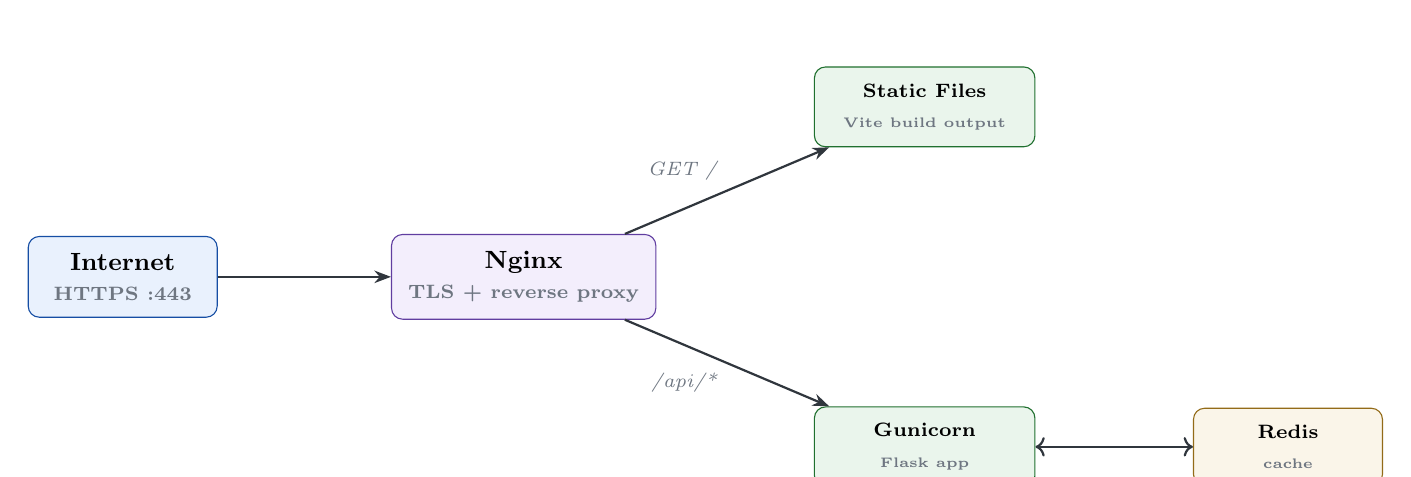
\begin{tikzpicture}[node distance=1.3cm and 2.2cm]

  \node[mynode=sectionblue, minimum width=2.4cm, minimum height=0.9cm] (internet)
    {\small Internet\\{\scriptsize\color{textmuted}HTTPS :443}};

  \node[mynode=accentpurple, minimum width=3.2cm, minimum height=1cm,
        right=2.2cm of internet] (nginx)
    {\small Nginx\\{\scriptsize\color{textmuted}TLS + reverse proxy}};

  \node[mynode=green, minimum width=2.8cm, minimum height=0.8cm,
        above right=1.1cm and 2cm of nginx] (static)
    {\scriptsize Static Files\\{\tiny\color{textmuted}Vite build output}};

  \node[mynode=green, minimum width=2.8cm, minimum height=0.8cm,
        below right=1.1cm and 2cm of nginx] (gunicorn)
    {\scriptsize Gunicorn\\{\tiny\color{textmuted}Flask app}};

  \node[mynode=amber, minimum width=2.4cm, minimum height=0.8cm,
        right=2cm of gunicorn] (redis)
    {\scriptsize Redis\\{\tiny\color{textmuted}cache}};

  \draw[arrow] (internet) -- (nginx);
  \draw[arrow] (nginx) -- node[lbl,above left]{GET /} (static);
  \draw[arrow] (nginx) -- node[lbl,below left]{/api/*} (gunicorn);
  \draw[arrow,<->] (gunicorn) -- (redis);

\end{tikzpicture}
\end{center}

\textbf{Recommended free-tier cloud options:}
\begin{itemize}
  \item \textbf{Railway.app} -- Backend (Gunicorn) + Redis as separate services; Vite build on Vercel.
  \item \textbf{Render.com} -- Web Service (Gunicorn) + Redis add-on. Spins down after 15 min of inactivity on free tier.
  \item \textbf{Fly.io} -- Docker-based deployment; generous free tier for always-on demos.
  \item \textbf{VPS (DigitalOcean / Hetzner)} -- \$4--6/month; full control with Docker Compose + Nginx + Certbot.
\end{itemize}

\newpage

%% ═══════════════════════════════════════════════════════════════════════════
\section{Project Summary Card}

\begin{center}
\begin{mdframed}[linecolor=border,linewidth=1pt,roundcorner=8pt,
                 innerleftmargin=24pt,innerrightmargin=24pt,
                 innertopmargin=16pt,innerbottommargin=16pt]
\begin{center}
{\large\bfseries\color{sectionblue} ARES CTI Dashboard -- Quick Reference}
\end{center}
\vspace{0.4cm}
\begin{tabular}{ll}
\textbf{Type}        & Full-Stack Web Application \\[3pt]
\textbf{Backend}     & Python 3.12 / Flask 3.0+ / flask-caching / requests \\[3pt]
\textbf{Frontend}    & React 18 / TypeScript / Vite / React Router / Recharts \\[3pt]
\textbf{Ext.\ APIs}  & AbuseIPDB, AlienVault OTX, VirusTotal \\[3pt]
\textbf{Cache}       & SimpleCache (dev) / Redis (prod) \\[3pt]
\textbf{Pattern}     & App factory, Blueprint per resource, Service layer \\[3pt]
\textbf{Concurrency} & ThreadPoolExecutor -- parallel API fan-out \\[3pt]
\textbf{IOC types}   & IP address, Domain, File hash (MD5/SHA256) \\[3pt]
\textbf{Endpoints}   & 8 REST endpoints \\[3pt]
\textbf{Pages}       & Dashboard, IOC Lookup, Threat Feed \\[3pt]
\textbf{Dev ports}   & Backend :5001 / Frontend :5173 \\
\end{tabular}
\end{mdframed}
\end{center}

\vspace{1.5cm}
\begin{center}
\color{textmuted}\small
Built by Rafael Rodriguez \quad \textbullet \quad April 2026 \\[4pt]
\href{https://github.com/rodriguezgonzalez}{github.com/rodriguezgonzalez}
\end{center}

\end{document}
